
Tables are made up of a number of columns. Each column must be assigned a name and a data type; within the table, each column name is unique, although it can be duplicated in another table.

.Here is an example of a simple table create statement for the DEPT table:

\ \ CREATE TABLE DEPT

\begin{center}
\begin{minipage}{2.249cm}
\begin{flushleft}
\tablefirsthead{}
\tablehead{}
\tabletail{}
\tablelasttail{}
\begin{supertabular}{|m{2.049cm}|}
\hline
\subsection[DEPT]{DEPT}
\\\hline
DEPTNO\\
DNAME\\
LOC\\\hline
\end{supertabular}
\end{flushleft}
\end{minipage}
\end{center}
\ \ \ \ ( DEPTNO\ \ \ \ NUMBER(2) ,

\ \ \ \  DNAME\ \ \ \ VARCHAR2(14) ,

\ \ \ \  LOC\ \ \ \ \ \ VARCHAR2(13)  ) ;

The parameters required to define the table (columns, constraints) are separated by a comma. The whole group of parameters is enclosed within a set of brackets. The create statement gives the system the information needed to set up a relational system; for that reason, a reader can work out the entity details from the table create statement, as for the DEPT table above.

E1. Draw the entity and attributes implemented by this create statement.



\begin{center}
\begin{minipage}{5.914cm}
\end{minipage}
\end{center}
\ \ CREATE TABLE CUST

\ \ \ \ ( CUSTNO\ \ \ \ CHAR(4) ,

\ \ \ \  NAME\ \ \ \ VARCHAR2(30) ,

\ \ \ \  ADDRESS\ \ \ \ VARCHAR2(50) ,

AREA\ \ \ \ \ \ VARCHAR2(10)  ) ;

This simple version of the CREATE statement does not define a primary key. This, and other integrity constrains, is dealt with later in the section. However, it is good practice to create {\textquotedbl}parent{\textquotedbl} tables before the {\textquotedbl}child{\textquotedbl} tables that depend on them, as if referential integrity was applicable.

\begin{center}
  

\includegraphics[width=1.06cm,height=0.903cm]{images/img (2).png}

\end{center}
\subsection[Naming Rules {}- to apply to table, view and columns names.]{Naming Rules - to apply to table, view and columns names.}
\begin{itemize}
\item must start with a letter.
\item may be between 1 and 30 characters long.
\item may contain alphabetic and numeric characters  A to Z, a to z, 0 to 9.
\item are not case sensitive
\item cannot be a reserved word
\item may contain underscores
\item may contain \$ and \#  (but not recommended)
\end{itemize}
\subsection[Choosing Data Types]{Choosing Data Types}
The main data types divide in three groups: numbers, text and date/time. The full detail of how each type is written, with examples, is  in the next page.

\begin{itemize}
\item The number type is intended to store numbers that are calculated on. They are not suitable, for example, for a telephone number or a numerical code, because these often have leading 0s and sometimes even non-numeric characters. But they are perfect for the number of products purchased or money earned -- which will certainly need the arithmetic.
\item Text types -- there are several -- are used for anything that requires characters. The different types depend on whether the data uses a fixed number of characters (for example, a post code), or an unpredictable text length.
\item Date and time -- in Oracle, both use the same data type. Internally, Oracle records this as a number. The integer part is the day (counting the days since approx. 6000 years ago) with the time as the decimal part.
\end{itemize}


\begin{center}
  

\includegraphics[width=1.06cm,height=0.903cm]{images/img (2).png}

\end{center}
Always enclose text and date data in single quote marks, 'like this'

The declaration of the data type determines the operations that may be performed on the data: e.g. when sorting, strings are sorted alphabetically (in ASCII code order), while number data is sorted numerically.

The main data types supported by the version of SQL used on the course are shown in the table below:-

\begin{flushleft}
\tablefirsthead{}
\tablehead{}
\tabletail{}
\tablelasttail{}
\begin{supertabular}{|m{3.552cm}|m{12.048cm}|}
\hline
Data Type &
Description\\\hline
CHAR(n) &
Fixed length character string of n characters. 0{\textless}n{\textless}2001, default n=1.

Single quote marks must be placed around any character string being inserted into or compared against a column of this type.\\\hline
VARCHAR2(n)

 &
Variable length character string, having a maximum length of n. 0{\textless}n{\textless}4001, no default value so n must be specified.

Single quote marks must be placed around any character string being inserted into or compared against a column of this type.\\\hline
DATE &
Dates ranging from 01/01/4712 BC to 31/12/4712 AD, and time.  Default time is midnight (12:00:00 AM).

Place single quote marks around any character string being inserted into or compared against a column of this type.\\\hline
NUMBER  &
A number, with 38 figures and no decimals.\ \ \\\hline
NUMBER(p, s) &
Where it is given, p is the total number of digits (between 1 and 38 included) and s the number of decimal places (between 0 and p included), e.g.

\ \ NUMBER(7,0) will store -99,999 to + 99,999

 NUMBER(5,2) will hold -999.99 to +999.99

 NUMBER(5,5) will hold -0.99999 to + 0.99999\\\hline
\end{supertabular}
\end{flushleft}
E2\ \ Create the three tables which implement the Accounting System that was described in the Introduction. (Note - column ACCNO will be defined as numeric.) 

\begin{flushleft}
\tablefirsthead{}
\tablehead{}
\tabletail{}
\tablelasttail{}
\begin{supertabular}{|m{14.663cm}|}
\hline
CREATE TABLE CUST

\ \ \ \ ( CUSTNO\ \ \ \ CHAR(4) ,

\ \ \ \  NAME\ \ \ \ VARCHAR2(30) ,

\ \ \ \  ADDRESS\ \ \ \ VARCHAR2(50) ,

AREA\ \ \ \ \ \ VARCHAR2(10)  ) ;

\\\hline
CREATE

\\\hline
CREATE

\\\hline
\end{supertabular}
\end{flushleft}
\section{The DROP statement}
This enables you to delete a table that already exists.

 DROP TABLE table\_name ;\ \ \ \ 



\begin{center}
  
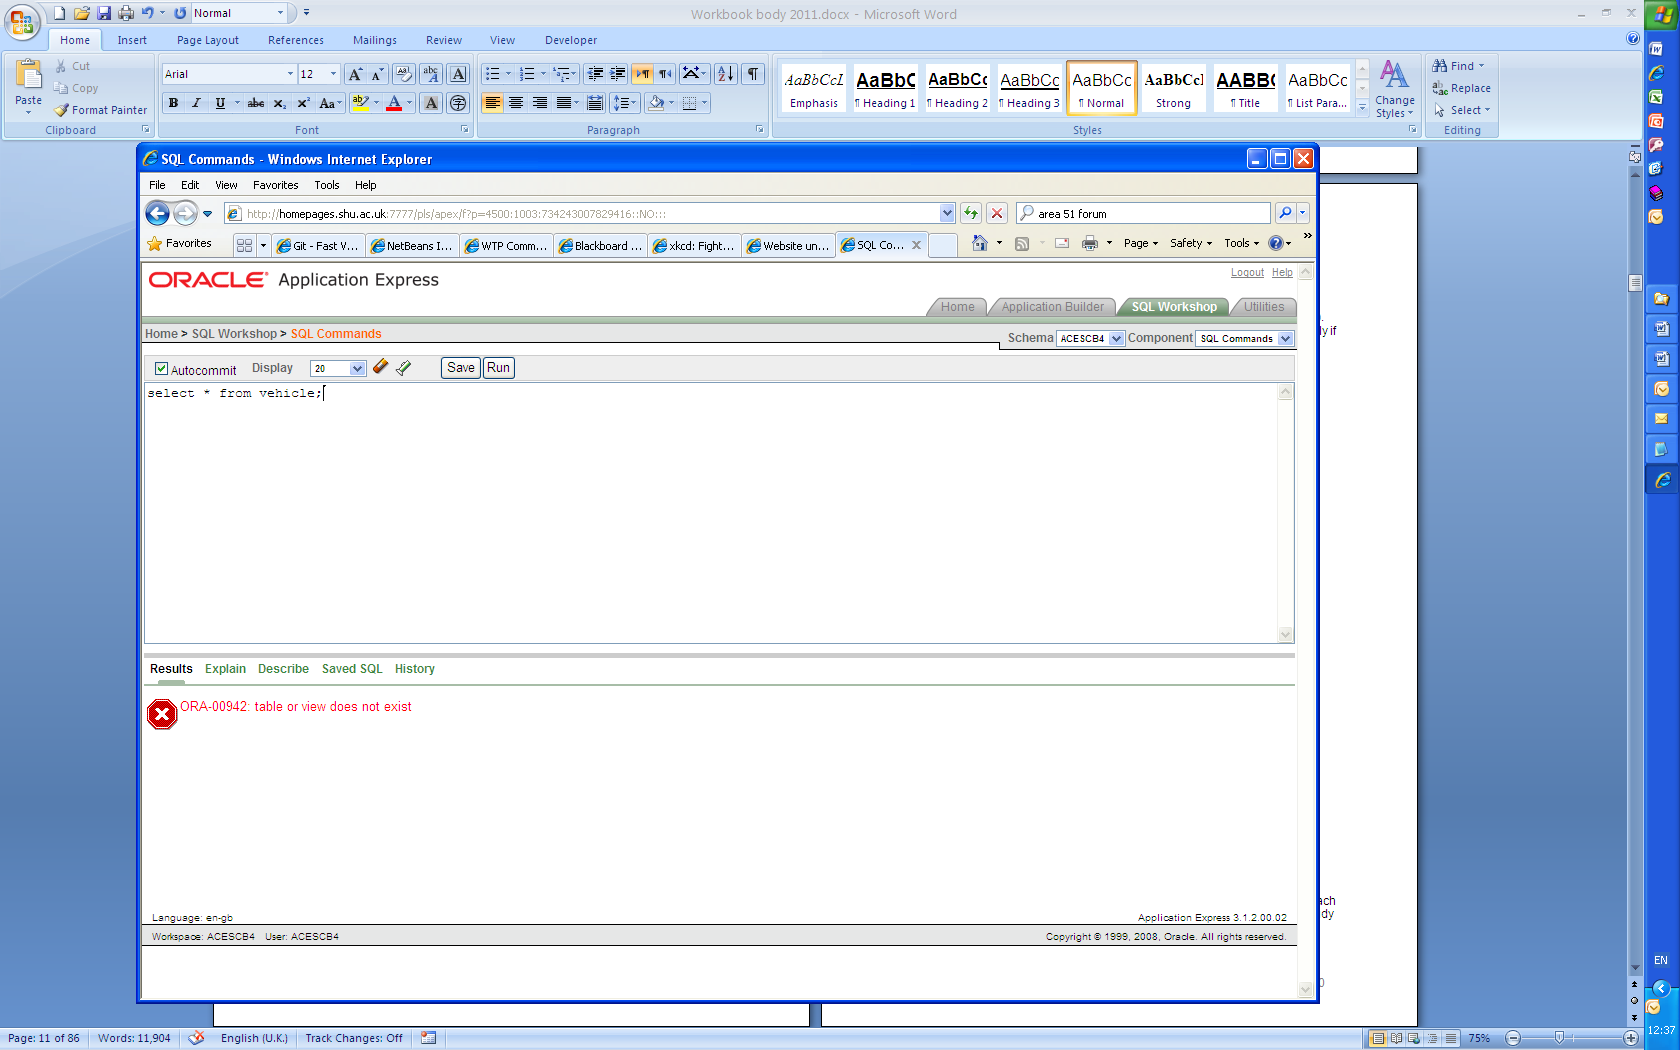
\includegraphics[width=8.449cm,height=2.644cm]{images/img (41).png}

\end{center}
e.g.\ \ DROP TABLE CUST ;

You can easily check that a table has been dropped by trying a command that uses it -- any SELECT. The error to the right will show.

\section{Oracle recyclebin}
Oracle 10g introduced the concept of the recyclebin.  Information about objects which have been dropped is placed in a recyclebin data dictionary table.  A dropped object will have an object name like BIN\$45azVqPcJrHgNAADugjeBA==\$0: 

To produce a list of all deleted tables with their original name:

\ \ SELECT * FROM RECYCLEBIN ;

To restore a table run the following command: 

\ \ FLASHBACK TABLE tablename TO BEFORE DROP ;

To permanently remove all of them run the following command: 

\ \ PURGE RECYCLEBIN ;

\clearpage
\section{The INSERT statement}
Values are inserted into a table one row at a time.

INSERT INTO DEPT

\ \ \ \ VALUES (60, 'PURCHASING', 'BOSTON') ;

This will enter a value into every column in one new row.  The values must be presented in the same sequence as the columns appear in the DESCRIBE command.



\begin{center}
  

\includegraphics[width=1.05cm,height=0.903cm]{images/img (2).png}

\end{center}
The single quote marks around character strings are mandatory; this also applies when entering dates.

Where the values to be used are in a different order to how they appear in the DESCRIBE command we specify the column names in the order of the values being entered.

\ \ INSERT INTO DEPT (DEPTNO, LOC, DNAME)

\ \ \ \ VALUES (50, `NEW YORK', `PERSONNEL') ;

We can also insert rows into a table with missing data values (value is NULL), provided we don't try to omit values which are defined as mandatory (not null), e.g. the primary key, but this will require us to specify the columns into which we are entering data.

\ \ INSERT INTO DEPT (DEPTNO)

\ \ \ \ VALUES (70) ;

This will insert a new row with department number set to 70 and the remaining columns will be left empty (null).

In general, insert takes the form

\ \ INSERT INTO\ \ table\_name ( column1 [ , ... ] )

\ \ VALUES \ \ \ \ ( field\_value1 [ , ... ] ) ;



\begin{center}
  

\includegraphics[width=1.076cm,height=0.917cm]{images/img (2).png}

\end{center}
Note that in Oracle, an INSERT statement can add only one row of data. 

This doesn't work: 

INSERT INTO DEPT VALUES

\begin{center}
  

\includegraphics[width=1.443cm,height=1.427cm]{images/img (26).png}

\end{center}
(50, `NEW YORK', `PERSONNEL'),

(90,'SAN FRANCISCO,'SALES') ;

Instead you should use these two separate statements:

INSERT INTO DEPT VALUES ( 50, `NEW YORK', `PERSONNEL' ) ;

\begin{center}
  

\includegraphics[width=1.443cm,height=1.184cm]{images/img (27).png}

\end{center}
INSERT INTO DEPT VALUES ( 90,'SAN FRANCISCO,'SALES{}' ) ;

In many programming languages the absence of a value (or parameter) is often indicated by placing two commas together.  It is not valid to indicate null values using this approach.  So, 

INSERT INTO DEPT

\begin{center}
  

\includegraphics[width=1.443cm,height=1.427cm]{images/img (26).png}

\end{center}
\ \ VALUES (70,,'BOSTON') ;

is an invalid way of trying to enter a null value for the department name.  The correct way is:

INSERT INTO DEPT

\begin{center}
  

\includegraphics[width=1.443cm,height=1.184cm]{images/img (27).png}

\end{center}
\ \ VALUES(70,NULL,'BOSTON') ;

\section{Inserting time and date data}
For Date columns:

\ \ INSERT INTO EMP (EMPno, Hiredate)

\ \ \ \ VALUES (999, '01-JAN-2001') ;

Columns defined as Date types hold both date and time values but normally the time element is ignored and not presented by a SELECT statement.  By default the time is set to 12.00 midnight.

To store a specific time in a date column we use the TO\_DATE function:

\ \ INSERT INTO ACC (ACCNO, OPENED)

\ \ VALUES (1245890, TO\_DATE('12-NOV-2003 10:10', 'dd-mon-yy hh:mi') ) ;

To see the time element we use the TO\_CHAR function with a string format made up of those shown in the appendix of this workbook.

\ \ SELECT ACCNO, TO\_CHAR(OPENED, 'dd-mon-yy hh:mi') 

\ \ from ACC

\ \ WHERE ACCNO = 1245890;

will display:

   
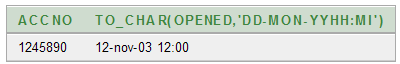
\includegraphics[width=10.576cm,height=1.706cm]{images/img (42).png}
 

More detail about these functions, and especially the possible string formats used with them, is in the appendix of this workbook.

E3\ \ Populate the Accounting System tables that you created in Exercise E2 with the data as given in the Introduction p. 7.  Give an example of one insert statement for each table in the boxes below.

\begin{flushleft}
\tablefirsthead{}
\tablehead{}
\tabletail{}
\tablelasttail{}
\begin{supertabular}{|m{14.663cm}|}
\hline
INSERT

\\\hline
INSERT

\\\hline
INSERT

\\\hline
\end{supertabular}
\end{flushleft}

\section{Create and run a Script}
Running individual statements is useful; but sometimes there are a series of instructions to be issued. Re-typing instructions is time-consuming, tedious, and error-prone.

The 'SQL Scripts' feature within the interface provides an alternative: a way of storing lists of instructions in files.  In addition you can upload scripts created in some other editor, and download scripts to use outside of the APEX interface.

Return to the SQL Workshop screen (Home{\textgreater}SQL Workshop) to select the SQL Scripts feature. Press the 'Create' button and give the script a name.



\begin{center}
  
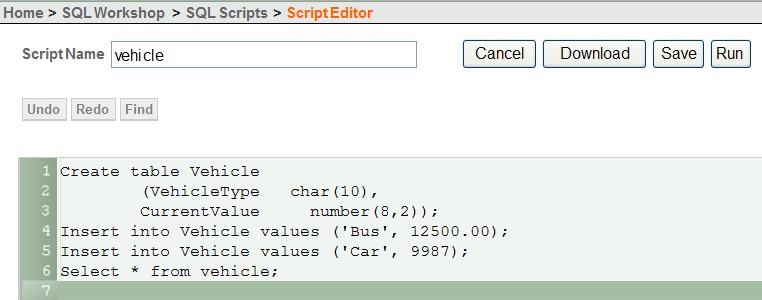
\includegraphics[width=14.727cm,height=5.068cm]{images/img (43).png}

\end{center}


\begin{center}
\begin{minipage}{3.133cm}
Name scripts
\end{minipage}
\end{center}


\begin{center}
\begin{minipage}{3.133cm}
Manage files
\end{minipage}
\end{center}


\begin{center}
\begin{minipage}{2.854cm}
Edit scripts online
\end{minipage}
\end{center}
In the editor, type the Create, Insert and Select statements used previously for the Vehicle table.

The semicolon is optional for single statements in `non-script' mode in APEX and SQLDeveloper, but it's still mandatory between multiple statements in `script' mode.

\begin{center}
  

\includegraphics[width=1.058cm,height=0.903cm]{images/img (2).png}

\end{center}
E4\ \ Type up the commands to create the Accounting System and populate the tables.

E5\ \ Run the script. A confirmation screen appears. Why is there such a high level of security managing these scripts? 

\begin{flushleft}
\tablefirsthead{}
\tablehead{}
\tabletail{}
\tablelasttail{}
\begin{supertabular}{|m{14.663cm}|}
\hline
\\\hline
\end{supertabular}
\end{flushleft}
Once the script has run, you are presented with a history of script results. Choose the 'Detail' option and press 'Go' to see the full results.

   
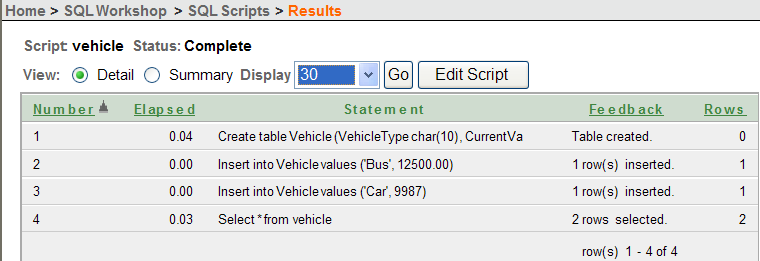
\includegraphics[width=14.748cm,height=4.094cm]{images/img (44).png}
 

You see details of each of the statements and the results from running them.  Take a few moments to study them; check that your script has run correctly.

Return to the SQL Scripts screen (Home{\textgreater}SQL Workshop{\textgreater}SQL Scripts).  Your named script has been saved within your Oracle environment.

E5\ \ Now create a second script for the Drop statements and run that.

\clearpage
\section{Editing scripts}

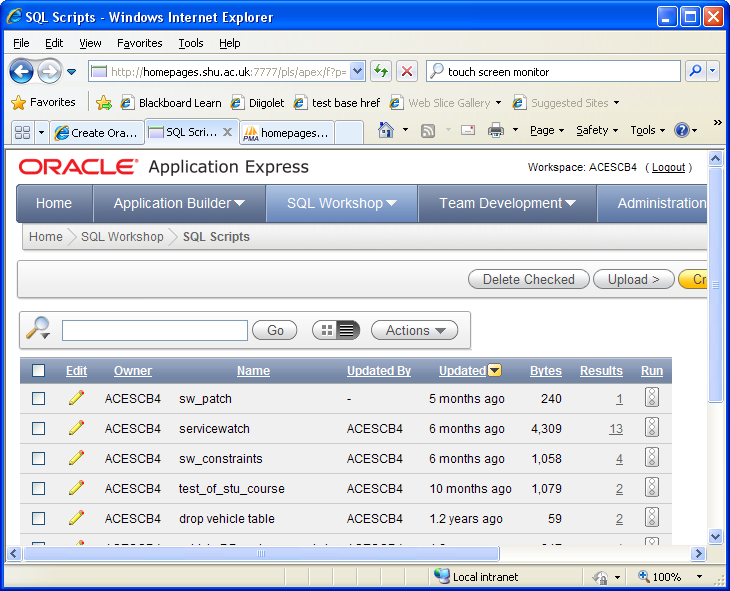
\includegraphics[width=14.9cm,height=3.108cm]{images/img (45).png}
 

The scripts you created are stored within the Oracle environment.  You can edit it a script in that environment by clicking on the pencil icon for that script, as shown above.

Alternatively, it is often convenient to prepare a script away from Oracle and then upload it for processing, or to download a stored script for editing outside of Oracle.

To manage your scripts and keep your environment tidy, you may want to move them to an appropriate folder in your work area.

\section{Downloading and Uploading scripts}
Download the vehicle script to your work area and save it as vehicle.sql (ensure it has a '.sql' extension). In a text editor, open the file. Use white space (the {\textless}Space{\textgreater}, {\textless}Enter{\textgreater}, and {\textless}Tab{\textgreater} characters) to make the statements clear. Save the file, ensuring its name and extension are correct.

Some editors, like notepad, add an extra .txt extension. You should find a better text editor than notepad -{}-{}- at least one that shows you line numbers, highlights SQL syntax in colour, and respects your choice of name extension

\begin{center}
  

\includegraphics[width=1.06cm,height=0.903cm]{images/img (2).png}

\end{center}
 when you save. A favourite is Notepad++ (http://notepad-plus-plus.org/).

Switch to the Oracle window and to the SQL Scripts option. Select 'Upload', locate the file you have just saved, and upload it.

\section{Commenting SQL scripts}
Comments can be included to clarify and explain an SQL statement or procedure. 

The comment starts with /* and ends with */, preferably on their own lines, e.g.

\ \ /*

 \ \ \ \ Comment out multiple full lines

\ \ \ \ placed between the start and end points 

\ \ */

To comment out single lines, use -{}- e.g.

\ \ {}-{}-  this line is a comment

\ \ DESCRIBE EMP -{}- this text after the dashes is a comment

\clearpage